\documentclass{article}
\usepackage{amsmath}
\usepackage{amssymb}
\usepackage{tikz}
\usetikzlibrary{patterns}

\begin{document}

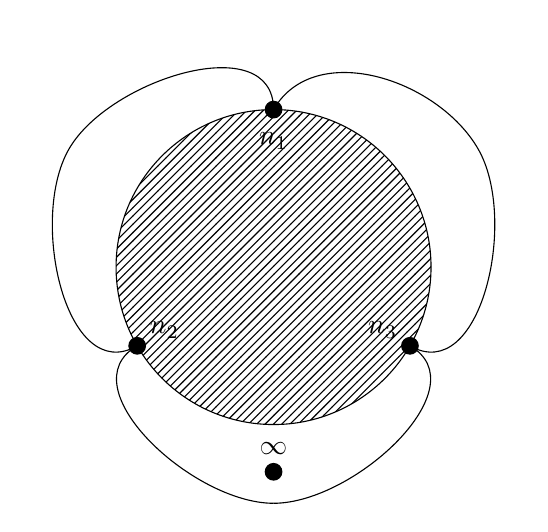
\begin{tikzpicture}
\draw[pattern = north east lines] (0, 0) circle (2);

\filldraw (1.732, -1) circle (3 pt);
\node at (1.386, -0.8) {$n_3$};
\filldraw (-1.732, -1) circle (3 pt);
\node at (-1.386, -0.8) {$n_2$};
\filldraw (0, 2) circle (3 pt);
\node at (0, 1.6) {$n_1$};

\draw (-1.732, -1) to[in = 180, out = 210] (0, -3);
\draw (0, -3) to[in = -30, out = 0] (1.732, -1);

\draw (1.732, -1) to[in = -60, out = -30] (2.598, 1.5);
\draw (2.598, 1.5) to[in = 60, out = 120] (0, 2);

\draw (0, 2) to[in = 60, out = 90] (-2.598, 1.5);
\draw (-2.598, 1.5) to[in = -150, out = -120] (-1.732, -1);

\filldraw (0, -2.6) circle (3 pt);
\node at (0, -2.3) {$\infty$};

\end{tikzpicture}

\end{document}